%iffalse
\let\negmedspace\undefined
\let\negthickspace\undefined
\documentclass[journal,12pt,onecolumn]{IEEEtran}
\usepackage{cite}
\usepackage{amsmath,amssymb,amsfonts,amsthm}
\usepackage{algorithmic}
\usepackage{graphicx}
\usepackage{textcomp}
\usepackage{xcolor}
\usepackage{txfonts}
\usepackage{listings}
\usepackage{enumitem}
\usepackage{mathtools}
\usepackage{gensymb}
\usepackage{comment}
\usepackage[breaklinks=true]{hyperref}
\usepackage{tkz-euclide} 
\usepackage{listings}
\usepackage{gvv}                                        
%\def\inputGnumericTable{}                                 
\usepackage[latin1]{inputenc}     
\usepackage{xparse}
\usepackage{color}                                            
\usepackage{array}                                            
\usepackage{longtable}                                       
\usepackage{calc}                                             
\usepackage{multirow}
\usepackage{multicol}
\usepackage{hhline}                                           
\usepackage{ifthen}                                           
\usepackage{lscape}
\usepackage{tabularx}
\usepackage{array}
\usepackage{float}
\newtheorem{theorem}{Theorem}[section]
\newtheorem{problem}{Problem}
\newtheorem{proposition}{Proposition}[section]
\newtheorem{lemma}{Lemma}[section]
\newtheorem{corollary}[theorem]{Corollary}
\newtheorem{example}{Example}[section]
\newtheorem{definition}[problem]{Definition}
\newcommand{\BEQA}{\begin{eqnarray}}
\newcommand{\EEQA}{\end{eqnarray}}
\newcommand{\define}{\stackrel{\triangle}{=}}
\theoremstyle{remark}
\newtheorem{rem}{Remark}
% Marks the beginning of the document
\begin{document}
\title{Assignment 3}
\author{EE24Btech11024 - G. Abhimanyu Koushik}
\maketitle
\renewcommand{\thefigure}{\theenumi}
\renewcommand{\thetable}{\theenumi}
\subsection{Multiple Choice}
\begin{enumerate}

\item Let $X$ be a random variable such that the probability function of a distribution given by $P\brak{X=0}=\frac{1}{2}$, $P\brak{X=j}=\frac{1}{3^j}$ $\brak{j=1,2,3,\dots,\infty}$. Then the mean of the distribution and $P\brak{X\text{ is positive and even}}$ respectively are:

\hfill{\brak{\text{Jul 2021}}}
\begin{enumerate}
\begin{multicols}{4}
\item $\frac{3}{8}$ and $\frac{1}{8}$
\item $\frac{3}{4}$ and $\frac{1}{8}$
\item $\frac{3}{4}$ and $\frac{1}{9}$
\item $\frac{3}{4}$ and $\frac{1}{16}$
\end{multicols}
\end{enumerate}

\item If the tangent to the ellipse $x^2+4y^2=4$ meets the tangents at the extremities of its major axis at $\vec{B}$ and $\vec{C}$, then the circle with $BC$ as diameter pass through the point:

\hfill{\brak{\text{Jul 2021}}}
\begin{enumerate}
\begin{multicols}{4}
\item $\brak{\sqrt{3},0}$
\item $\brak{\sqrt{2},0}$
\item $\brak{1,1}$
\item $\brak{-1,1}$
\end{multicols}
\end{enumerate}

\item Let the equation of pair of lines , $y=px$ and $y=qx$, can be written as $\brak{y-px}\brak{y-qx}=0$. Then the equation of the pair of angle bisectors of the lines $x^2-4xy-5y^2=0$ is:

\hfill{\brak{\text{Jul 2021}}}
\begin{enumerate}
\begin{multicols}{4}
\item $x^2-3xy+y^2=0$
\item $x^2+4xy-y^2=0$
\item $x^2+3xy-y^2=0$
\item $x^2-3xy-y^2=0$
\end{multicols}
\end{enumerate}

\item If $\perm{n}{r}=\perm{n}{r+1}$ and $\comb{n}{r} = \comb{n}{r+1}$, then the value of $r$ is equal to:
\hfill{\brak{\text{Jul 2021}}}
\begin{enumerate}
\begin{multicols}{4}
\item $1$
\item $4$
\item $2$
\item $3$
\end{multicols}
\end{enumerate}

\item Let $y=y\brak{x}$ be the solution of the differential equation $xdy=\brak{y+x^{3}\cos x}dx$ with $y\brak{\pi}=0$, then $y\brak{\frac{\pi}{2}}$ is equal to:

\hfill{\brak{\text{Jul 2021}}}
\begin{enumerate}
\begin{multicols}{4}
\item $\frac{\pi^2}{4}+\frac{\pi}{2}$
\item $\frac{\pi^2}{2}+\frac{\pi}{4}$
\item $\frac{\pi^2}{2}-\frac{\pi}{4}$
\item $\frac{\pi^2}{4}-\frac{\pi}{2}$
\end{multicols}
\end{enumerate}
\end{enumerate}

\subsection{Numericals}
\begin{enumerate}

\item Let $n\in \mathbb{N}$ and $\sbrak{x}$ denote the greatest integer less than or equal to $x$. If the sum of $\brak{n+1}$ terms $\comb{n}{0}$, $3\cdot\comb{n}{1}$, $5\cdot\comb{n}{2}$, $7\cdot\comb{n}{3} \dots$ is equal to $2^{100}\cdot 101$, then $2\sbrak{\frac{n-1}{2}}$ is equal to \rule{1cm}{0.15mm}.

\hfill{\brak{\text{Jul 2021}}}

\item Consider the function $f\brak{x} = \begin{cases} \frac{P\brak{x}}{\sin\brak{x-2}} & x\neq 2, \\7 & x=2 .\end{cases}$ where $P\brak{x}$ is a polynomial such that ${P^\prime}^\prime\brak{x}$ is always a constant and $P\brak{3}=9$. If $f\brak{x}$ is continuous at $x=2$, then $P\brak{5}$ is equal to \rule{1cm}{0.15mm}.

\hfill{\brak{\text{Jul 2021}}}

\item The equation of a circle is $Re\brak{z^2}+2\brak{Im\brak{z}}^2+2Re\brak{z}=0$, where $z=x+iy$. A line which passes through the centre of the given circle and the vertex of parabola, $x^2-6x-y+13=0$, has y-intercept equal to \rule{1cm}{0.15mm}.

\hfill{\brak{\text{Jul 2021}}}

\item If a rectangle is inscribed in an equilateral triangle of side length $2\sqrt{2}$ as shown in the figure, then the square of the largest area of such a rectangle is \rule{1cm}{0.15mm}.
\\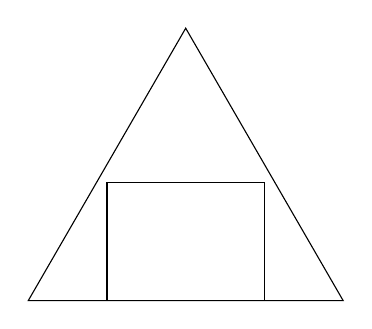
\begin{tikzpicture}
    \draw (0,0) -- (4,0) -- (2,3.46) -- cycle;
    \draw (1,0) -- (1,1.5) -- (3,1.5) -- (3,0);
\end{tikzpicture}

\hfill{\brak{\text{Jul 2021}}}

\item If $\brak{\vec{a}+3\vec{b}}$ is perpendicular to $\brak{7\vec{a}-5\vec{b}}$ and $\brak{\vec{a}-4\vec{b}}$ is perpendicular to $\brak{7\vec{a}-2\vec{b}}$, then the angle between $\vec{a}$ and $\vec{b}$ \brak{\text{in degrees}} is \rule{1cm}{0.15mm}.

\hfill{\brak{\text{Jul 2021}}}

\item Let a curve $y=f\brak{x}$ pass through the point $\brak{2,\brak{\log_e{2}}^2}$ and have slope $\frac{2y}{x\log_e{x}}$ for all positive real values of $x$. Then the value of $f\brak{e}$ is equal to \rule{1cm}{0.15mm}.

\hfill{\brak{\text{Jul 2021}}}

\item If $a+b+c=1$, $ab+bc+ca=2$ and $abc=3$, then the value of $a^4+b^4+c^4$ is equal to \rule{1cm}{0.15mm}.

\hfill{\brak{\text{Jul 2021}}}

\item A fair coin is tossed $n$-times such that the probability of getting at least one head is at least $0.9$. Then the minimum value of $n$ is \rule{1cm}{0.15mm}. 

\hfill{\brak{\text{Jul 2021}}}

\item If the co-efficient of $x^7$ and $x^8$ in the expansion of $\brak{2+\frac{x}{3}}^n$ are equal, then the value of n is equal to \rule{1cm}{0.15mm}.

\hfill{\brak{\text{Jul 2021}}}

\item If the lines $\frac{x-k}{1}=\frac{y-2}{2}=\frac{z-3}{3}$ and $\frac{x+1}{3}=\frac{y+2}{2}=\frac{z+3}{1}$ are co-planar then, the value of $k$ is \rule{1cm}{0.15mm}.

\hfill{\brak{\text{Jul 2021}}}

\end{enumerate}
\end{document}

